\begin{center}
  \textsf{Листок 4.}
\end{center}
\vspace{0.01mm}
\nopagebreak[4]
\taskpic{К свободному концу нити, прикреплённой к стене и перекинутой
  через блок, подвешен груз. Блок закреплён на бруске массы $m_0$,
  который может скользить по горизонтальной плоскости без трения. В
  начальный момент нить с грузом отклоняют от вертикального положения
  на угол $\alpha$ и затем отпускают. Определите ускорение бруска, если
  угол, образованный нитью с вертикалью, не меняется при движении
  системы. Чему равна масса груза.  }{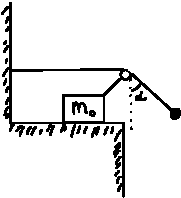
\includegraphics[width=4cm]{p09_13.pdf}}

\task{Где находится центр масс: однородного прута, согнутого
  посередине под прямым углом; однородной треугольной пластинки;
  гардеробного номерка в виде диска с круглым отверстием.  }

\taskpic{ Обезьяна массы $m$ уравновешена противовесом на блоке $A$. Блок $A$
  уравновешен грузом массы $2m$ на блоке $B$. Система неподвижна. Как
  будет двигаться груз, если обезьяна начнёт равномерно выбирать
  верёвку со скоростью $V$ относительно себя? Массой блоков и трением
  пренебречь.}{
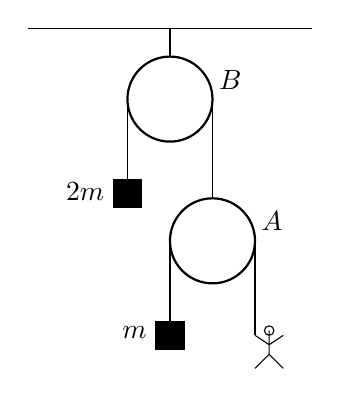
\begin{tikzpicture}[scale=0.6]
% потолок
  \draw (0,0) -- (6,0) (3,0) -- (3,-1.5);
% блок B
  \filldraw[thick,white,draw=black] (3,-1.5) circle (0.9)
  node[black,above=7,right=14] {$B$};
% верёвка к грузу 2m
  \draw (2.1,-1.5) -- ++(0,-2);
% груз 2m
  \filldraw[black] (1.8,-3.2) rectangle ++(0.6,-0.6)
  node[above=6,left=10] {$2m$};
% верёвка к блоку A
  \draw (3.9,-1.5) -- ++(0,-3);
% блок A
  \filldraw[thick,white,draw=black] (3.9,-4.5) circle (0.9)
  node[black,above=7,right=14] {$A$};;
% верёвки от блока A
  \draw (3,-4.5) -- ++(0,-2);
  \draw (4.8,-4.5) -- ++(0,-2);
% груз m
  \filldraw[black] (2.7,-6.2) rectangle ++(0.6,-0.6)
  node[above=6,left=10] {$m$};
% обезьяна
  \draw (4.8,-6.5) -- ++(0.3,-0.2) -- ++(0.3,0.2) ++(-0.3,-0.2) -- ++
  (0,0.3) circle (0.1) -- ++(0,-0.5) -- ++(0.3,-0.3) ++ (-0.3,0.3) --
  ++(-0.3,-0.3);
\end{tikzpicture}
%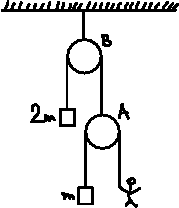
\includegraphics[width=4cm]{p09_15.pdf}
}

\task{ С какой силой давит на землю кобра, когда она, готовясь к
  прыжку, поднимается вертикально вверх с постоянной скоростью $V$?
  Масса змеи $m$, её длина $l$.  }
